\documentclass{article}
\usepackage[table,xcdraw]{xcolor}
\PassOptionsToPackage{table}{xcolor}
\usepackage[utf8]{inputenc}
\usepackage[framemethod=tikz]{mdframed}
\usepackage{physics}
\usepackage{amsmath}
\usepackage{tikz}
\usepackage{mathdots}
\usepackage{yhmath}
\usepackage{cancel}
\usepackage{color}
\usepackage{siunitx}
\usepackage{array}
\usepackage{multirow}
\usepackage{amssymb}
\usepackage{gensymb}
\usepackage{tabularx}
\usepackage{extarrows}
\usepackage{booktabs}
\usetikzlibrary{fadings}
\usetikzlibrary{patterns}
\usetikzlibrary{shadows.blur}
\usetikzlibrary{shapes}
\usepackage{float}
\usepackage{soul}


\title{Predictive Test Selection - Red Hat Inc.}
\author{Alon Mannor, Rubi Arviv}
\date{Submitted as final project report for Projects with the industry workshop, IDC, 2021}

\usepackage{natbib}
\usepackage{graphicx}

\begin{document}

\maketitle

\section{Introduction}

With ever increasing code repositories and tests needed to cover said code, the need for test prioritization schemes (i.e. producing a prioritized list of test to run, given a new code change) is becoming ever more essential. Various ways have been proposed to deterministically select which tests to run given a code change (for further details see the introduction section of the FB article, see below) .

A non-deterministic and promising approach is to use an ML-based model that will be trained on past code deployment runs, that contain code changes and the tests that ran as part of their deployment cycle. Given the historical data, such a model will be given a code change and a list of potential tests. It'll produce a prioritized list of the tests - from most likely to fail - to least likely. 

We have partnered with Red Hat to implement the approach provided in the FB article. The project chosen is Red Hat OpenShift.

\subsection{Related Works}
This project is based on a Facebook article by Machalica et al (hereinafter "the FB article").
\cite{MachalicaSP019}


\section{Solution}
\subsection{General approach}
We plan to go over the historical output of the CI and the OpenShift's GitHub repository. From these 2 sources, we'll scrape the historical raw data (containing things like all the metadata of CI deployments, test results, historical changes made to the project's files and more).
After having enough raw data, we'll run it through one or more stages of pre-processing and eventually use it to train an xgboost-based model. 
From there, we'll run both a classifier (outputting a binary fail/success prediction for a specific test) and a regressor (outputting a probability that a test will fail). In the latter approach, we'll use a cut-off value to be the threshold from which we recommend to run the test for a given code change (e.g. all the tests that have at least 80\% chance of failing).

There are many alternative approaches we tried, the main ones are:

\underline{In data scraping}: The project's CI output identifies a test by it's "locator" (a string value which can be thought of as the macro command use to run the test in the CI system). The task of mapping between the locator and the file/s that hold the test's code was no small feat. This required many cycles of trial-and-error. Eventually we decided to implement a straight-forward approach of iterating through the output's xml nodes, finding the one that holds the locator and looking at the node's text to look for any URLs starting the project's GitHub repo address.

\underline{In data analysis}: An important question we faced was whether to use a binary classifier or a regressor. The FB article used a regressor and 2 hyperparameters to calculate adhoc metrics (to asses how well the model performed). We implemented both a classifier and a regressor. We used off-the-shelf metrics (e.g. precision, recall, F1 score etc.). The classifier implementation produced results which weren't so good - so we implemented the regressor (with a final cutoff value of 0.7) - which improved the results.


In addition, there's a theoretical alternative we initially considered on how to get enough data. The idea was to deploy OpenShift on our own built environments and to introduce small  changes (that'll break the code) ourselves in order to produce known results (i.e. that a lot of tests would fail). This was rejected for a host of reasons, e.g. that deploying such a system can be painstakingly long and tedious, the code changes we'll introduce will be very simplistic and unnatural (since we don't have knowledge in the domain of the code, we would have done things like breaking compilation in a inelegant ways). Furthermore, we saw that the real-world data is good enough, in both quantity and quality.



\subsection{Data set}
We scraped data from 2 sources:

1) The OpenShift GitHub repo, located at: 
        \begin{verbatim}
        https://github.com/openshift/origin
        \end{verbatim}
2) The OpenShift CI dashboard, located at:
        \begin{verbatim}
        https://prow.ci.openshift.org/
        \end{verbatim}


We performed a pre-preprocessing step on these 2 (raw) data sources and produced the following 3 datasets:

i) \underline{Mapping changesets to tests}: Each test is identified by it's locator and also has the result of the specific run (i.e. "success" or "fail" - other state like "skipped" are ignored).

ii ) \underline{Mapping test locators to path/s}: As aforementioned, we used heuristics to deduce this mapping. We weren't successful in all of the times and some mapping are empty.

iii) \underline{Files changes history}: We used GitHub's API to scrape the project's repo and created a list of all the project's files and their changes (i.e. commits) history.

\subsection{Design}
The design is as follows, currently there is a scraping process to collect raw data from CI (to collect code change to test name, and test locator data) and GitHub (to collect changes history). This raw data is then aggregated into a flattened json file. Since xgboost can't handle raw text, in this stage we also encoded these fields. The flattened json is then translated to a CSV file using a customable configuration file. The CSV file is the input for the XGBoost regressor. The prediction's input  will be the changeset and the set of tests (each with either a 1 or 0, representing if the test has failed or succeeded, respectively). We will also include a cut-off parameter (a number between 0 and 1) that will decide whether the result is to to take the test or not with the current change that have been made. 
As been mentioned previously, the model that was selected is the xgboost regressor because the purpose is to decide whether a test should be selected for the changeset that have been made with a level of confidence (at the end we can't run all the tests, just the ones with a higher probability to fail). That is why the model returns a value between 0 and 1. A cut off parameter will decide whether a test has a high probability to be related to the change and we are not just interested just in returning \textit{True} or \textit{False}. This is why logistic regression was not used here.  
See Figure~\ref{fig:design} for the predictive test selection pipeline design.

%%%%%%%%%%%%%%%%%%%%%%%%%%%%%%%%%%%%%%%%%%%%%%%%%%%
% figure design
\begin{figure}
\centerline{\scalebox{0.75}{


\tikzset{every picture/.style={line width=0.75pt}} %set default line width to 0.75pt        

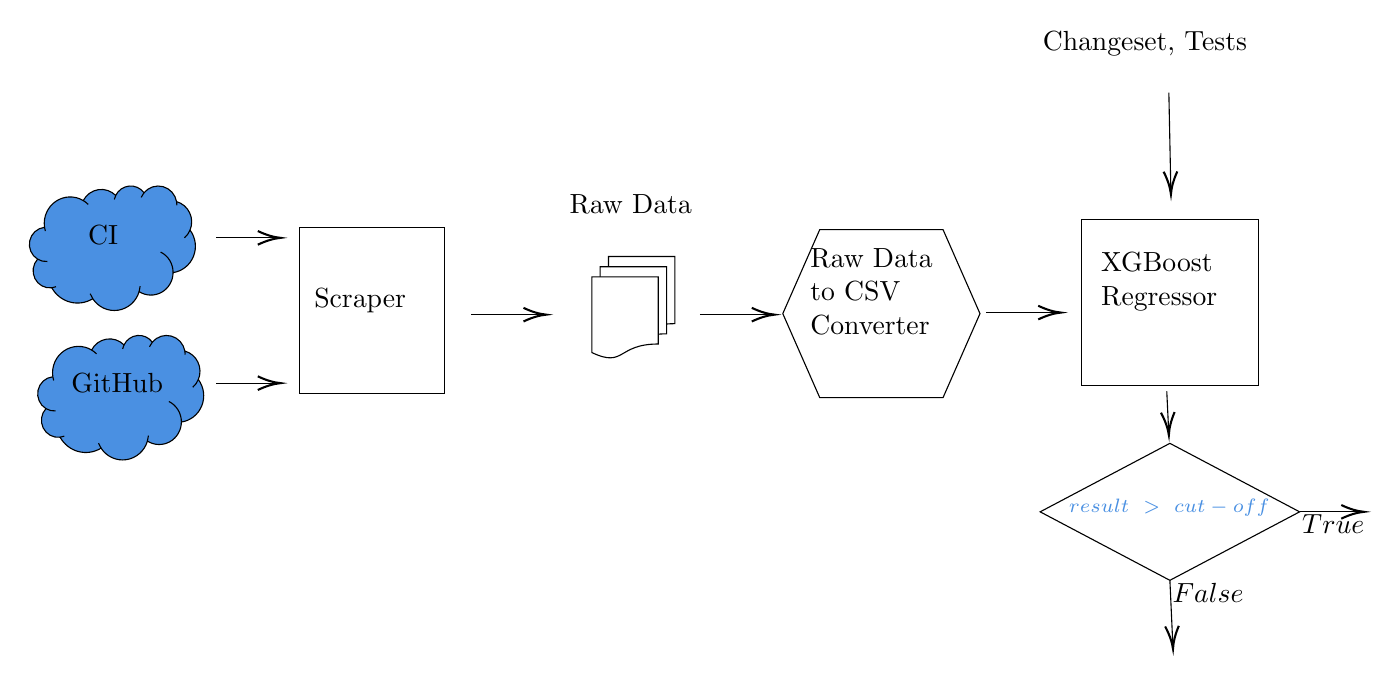
\begin{tikzpicture}[x=0.75pt,y=0.75pt,yscale=-1,xscale=1]
%uncomment if require: \path (0,340); %set diagram left start at 0, and has height of 340

%Shape: Cloud [id:dp9609078327942753] 
\draw  [fill={rgb, 255:red, 74; green, 144; blue, 226 }  ,fill opacity=1 ] (11.28,95.75) .. controls (10.64,90.92) and (12.75,86.13) .. (16.73,83.42) .. controls (20.7,80.71) and (25.85,80.56) .. (29.97,83.03) .. controls (31.43,80.21) and (34.1,78.27) .. (37.18,77.79) .. controls (40.26,77.3) and (43.38,78.33) .. (45.6,80.57) .. controls (46.84,78.02) and (49.29,76.31) .. (52.06,76.04) .. controls (54.84,75.77) and (57.55,76.98) .. (59.24,79.25) .. controls (61.49,76.55) and (65.07,75.41) .. (68.42,76.33) .. controls (71.78,77.25) and (74.32,80.06) .. (74.93,83.55) .. controls (77.69,84.31) and (79.98,86.27) .. (81.22,88.9) .. controls (82.47,91.53) and (82.53,94.58) .. (81.41,97.27) .. controls (84.12,100.88) and (84.75,105.68) .. (83.07,109.89) .. controls (81.39,114.11) and (77.65,117.09) .. (73.24,117.74) .. controls (73.21,121.69) and (71.09,125.32) .. (67.7,127.22) .. controls (64.3,129.12) and (60.16,129.01) .. (56.88,126.91) .. controls (55.48,131.65) and (51.54,135.13) .. (46.76,135.86) .. controls (41.99,136.59) and (37.23,134.43) .. (34.55,130.32) .. controls (31.26,132.34) and (27.31,132.93) .. (23.59,131.94) .. controls (19.88,130.95) and (16.71,128.46) .. (14.8,125.05) .. controls (11.44,125.45) and (8.19,123.67) .. (6.67,120.59) .. controls (5.14,117.51) and (5.66,113.79) .. (7.98,111.27) .. controls (4.98,109.47) and (3.45,105.89) .. (4.18,102.4) .. controls (4.92,98.92) and (7.76,96.31) .. (11.21,95.94) ; \draw   (7.98,111.27) .. controls (9.39,112.13) and (11.03,112.51) .. (12.66,112.38)(14.8,125.05) .. controls (15.51,124.96) and (16.2,124.79) .. (16.85,124.52)(34.55,130.32) .. controls (34.05,129.56) and (33.64,128.75) .. (33.31,127.9)(56.88,126.91) .. controls (57.13,126.05) and (57.3,125.16) .. (57.37,124.26)(73.24,117.74) .. controls (73.28,113.53) and (70.94,109.67) .. (67.23,107.83)(81.41,97.27) .. controls (80.81,98.7) and (79.89,99.97) .. (78.73,100.98)(74.93,83.55) .. controls (75.04,84.12) and (75.08,84.71) .. (75.07,85.3)(59.24,79.25) .. controls (58.68,79.92) and (58.22,80.68) .. (57.87,81.49)(45.6,80.57) .. controls (45.3,81.18) and (45.08,81.83) .. (44.93,82.5)(29.97,83.03) .. controls (30.84,83.55) and (31.65,84.18) .. (32.37,84.9)(11.28,95.75) .. controls (11.37,96.42) and (11.51,97.08) .. (11.7,97.72) ;

%Shape: Cloud [id:dp11776858327307993] 
\draw  [fill={rgb, 255:red, 74; green, 144; blue, 226 }  ,fill opacity=1 ] (15.28,167.75) .. controls (14.64,162.92) and (16.75,158.13) .. (20.73,155.42) .. controls (24.7,152.71) and (29.85,152.56) .. (33.97,155.03) .. controls (35.43,152.21) and (38.1,150.27) .. (41.18,149.79) .. controls (44.26,149.3) and (47.38,150.33) .. (49.6,152.57) .. controls (50.84,150.02) and (53.29,148.31) .. (56.06,148.04) .. controls (58.84,147.77) and (61.55,148.98) .. (63.24,151.25) .. controls (65.49,148.55) and (69.07,147.41) .. (72.42,148.33) .. controls (75.78,149.25) and (78.32,152.06) .. (78.93,155.55) .. controls (81.69,156.31) and (83.98,158.27) .. (85.22,160.9) .. controls (86.47,163.53) and (86.53,166.58) .. (85.41,169.27) .. controls (88.12,172.88) and (88.75,177.68) .. (87.07,181.89) .. controls (85.39,186.11) and (81.65,189.09) .. (77.24,189.74) .. controls (77.21,193.69) and (75.09,197.32) .. (71.7,199.22) .. controls (68.3,201.12) and (64.16,201.01) .. (60.88,198.91) .. controls (59.48,203.65) and (55.54,207.13) .. (50.76,207.86) .. controls (45.99,208.59) and (41.23,206.43) .. (38.55,202.32) .. controls (35.26,204.34) and (31.31,204.93) .. (27.59,203.94) .. controls (23.88,202.95) and (20.71,200.46) .. (18.8,197.05) .. controls (15.44,197.45) and (12.19,195.67) .. (10.67,192.59) .. controls (9.14,189.51) and (9.66,185.79) .. (11.98,183.27) .. controls (8.98,181.47) and (7.45,177.89) .. (8.18,174.4) .. controls (8.92,170.92) and (11.76,168.31) .. (15.21,167.94) ; \draw   (11.98,183.27) .. controls (13.39,184.13) and (15.03,184.51) .. (16.66,184.38)(18.8,197.05) .. controls (19.51,196.96) and (20.2,196.79) .. (20.85,196.52)(38.55,202.32) .. controls (38.05,201.56) and (37.64,200.75) .. (37.31,199.9)(60.88,198.91) .. controls (61.13,198.05) and (61.3,197.16) .. (61.37,196.26)(77.24,189.74) .. controls (77.28,185.53) and (74.94,181.67) .. (71.23,179.83)(85.41,169.27) .. controls (84.81,170.7) and (83.89,171.97) .. (82.73,172.98)(78.93,155.55) .. controls (79.04,156.12) and (79.08,156.71) .. (79.07,157.3)(63.24,151.25) .. controls (62.68,151.92) and (62.22,152.68) .. (61.87,153.49)(49.6,152.57) .. controls (49.3,153.18) and (49.08,153.83) .. (48.93,154.5)(33.97,155.03) .. controls (34.84,155.55) and (35.65,156.18) .. (36.37,156.9)(15.28,167.75) .. controls (15.37,168.42) and (15.51,169.08) .. (15.7,169.72) ;

%Shape: Rectangle [id:dp13008203036034538] 
\draw   (134,96) -- (204,96) -- (204,176) -- (134,176) -- cycle ;
%Straight Lines [id:da6622319456918209] 
\draw    (94,171) -- (123,171) ;
\draw [shift={(125,171)}, rotate = 180] [color={rgb, 255:red, 0; green, 0; blue, 0 }  ][line width=0.75]    (10.93,-3.29) .. controls (6.95,-1.4) and (3.31,-0.3) .. (0,0) .. controls (3.31,0.3) and (6.95,1.4) .. (10.93,3.29)   ;
%Straight Lines [id:da8919883280106733] 
\draw    (94,101) -- (123,101) ;
\draw [shift={(125,101)}, rotate = 180] [color={rgb, 255:red, 0; green, 0; blue, 0 }  ][line width=0.75]    (10.93,-3.29) .. controls (6.95,-1.4) and (3.31,-0.3) .. (0,0) .. controls (3.31,0.3) and (6.95,1.4) .. (10.93,3.29)   ;
%Flowchart: Multidocument [id:dp4714572678205542] 
\draw  [fill={rgb, 255:red, 255; green, 255; blue, 255 }  ,fill opacity=1 ] (283,110) -- (315,110) -- (315,142.34) .. controls (295,142.34) and (299,154) .. (283,146.46) -- cycle ; \draw  [fill={rgb, 255:red, 255; green, 255; blue, 255 }  ,fill opacity=1 ] (279,114.9) -- (311,114.9) -- (311,147.24) .. controls (291,147.24) and (295,158.9) .. (279,151.36) -- cycle ; \draw  [fill={rgb, 255:red, 255; green, 255; blue, 255 }  ,fill opacity=1 ] (275,119.8) -- (307,119.8) -- (307,152.14) .. controls (287,152.14) and (291,163.8) .. (275,156.26) -- cycle ;
%Straight Lines [id:da35684022665665305] 
\draw    (217,138) -- (251,138) ;
\draw [shift={(253,138)}, rotate = 180] [color={rgb, 255:red, 0; green, 0; blue, 0 }  ][line width=0.75]    (10.93,-3.29) .. controls (6.95,-1.4) and (3.31,-0.3) .. (0,0) .. controls (3.31,0.3) and (6.95,1.4) .. (10.93,3.29)   ;
%Straight Lines [id:da46505550523122463] 
\draw    (327,138) -- (361,138) ;
\draw [shift={(363,138)}, rotate = 180] [color={rgb, 255:red, 0; green, 0; blue, 0 }  ][line width=0.75]    (10.93,-3.29) .. controls (6.95,-1.4) and (3.31,-0.3) .. (0,0) .. controls (3.31,0.3) and (6.95,1.4) .. (10.93,3.29)   ;
%Shape: Rectangle [id:dp06068663083652348] 
\draw   (511,92) -- (596.14,92) -- (596.14,172) -- (511,172) -- cycle ;

%Straight Lines [id:da8952889351026803] 
\draw    (465,137) -- (499,137) ;
\draw [shift={(501,137)}, rotate = 180] [color={rgb, 255:red, 0; green, 0; blue, 0 }  ][line width=0.75]    (10.93,-3.29) .. controls (6.95,-1.4) and (3.31,-0.3) .. (0,0) .. controls (3.31,0.3) and (6.95,1.4) .. (10.93,3.29)   ;
%Straight Lines [id:da4741970161978426] 
\draw    (553,31) -- (553.96,78) ;
\draw [shift={(554,80)}, rotate = 268.83] [color={rgb, 255:red, 0; green, 0; blue, 0 }  ][line width=0.75]    (10.93,-3.29) .. controls (6.95,-1.4) and (3.31,-0.3) .. (0,0) .. controls (3.31,0.3) and (6.95,1.4) .. (10.93,3.29)   ;
%Flowchart: Preparation [id:dp8906764077543841] 
\draw   (367,137.5) -- (384.81,97) -- (444.19,97) -- (462,137.5) -- (444.19,178) -- (384.81,178) -- cycle ;

%Flowchart: Decision [id:dp9974841699132762] 
\draw   (553.5,200) -- (616,233) -- (553.5,266) -- (491,233) -- cycle ;
%Straight Lines [id:da9882816910535202] 
\draw    (552,175) -- (552.9,194) ;
\draw [shift={(553,196)}, rotate = 267.27] [color={rgb, 255:red, 0; green, 0; blue, 0 }  ][line width=0.75]    (10.93,-3.29) .. controls (6.95,-1.4) and (3.31,-0.3) .. (0,0) .. controls (3.31,0.3) and (6.95,1.4) .. (10.93,3.29)   ;
%Straight Lines [id:da8971663601544779] 
\draw    (616,233) -- (645,233) ;
\draw [shift={(647,233)}, rotate = 180] [color={rgb, 255:red, 0; green, 0; blue, 0 }  ][line width=0.75]    (10.93,-3.29) .. controls (6.95,-1.4) and (3.31,-0.3) .. (0,0) .. controls (3.31,0.3) and (6.95,1.4) .. (10.93,3.29)   ;
%Straight Lines [id:da5491567348239237] 
\draw    (553.5,266) -- (554.91,297) ;
\draw [shift={(555,299)}, rotate = 267.4] [color={rgb, 255:red, 0; green, 0; blue, 0 }  ][line width=0.75]    (10.93,-3.29) .. controls (6.95,-1.4) and (3.31,-0.3) .. (0,0) .. controls (3.31,0.3) and (6.95,1.4) .. (10.93,3.29)   ;


% Text Node
\draw (553.5,266) node [anchor=north west][inner sep=0.75pt]    {$False$};
% Text Node
\draw (616,233) node [anchor=north west][inner sep=0.75pt]    {$True$};
% Text Node
\draw (553.22,231) node  [font=\scriptsize,color={rgb, 255:red, 74; green, 144; blue, 226 }  ,opacity=1 ]  {$result\  >\ cut-off$};
% Text Node
\draw (491,0) node [anchor=north west][inner sep=0.75pt]   [align=left] {Changeset, Tests};
% Text Node
\draw (263,79) node [anchor=north west][inner sep=0.75pt]   [align=left] {Raw Data};
% Text Node
\draw (140,124) node [anchor=north west][inner sep=0.75pt]   [align=left] {Scraper};
% Text Node
\draw (379,105) node [anchor=north west][inner sep=0.75pt]   [align=left] {Raw Data \\to CSV \\Converter};
% Text Node
\draw (519.11,107) node [anchor=north west][inner sep=0.75pt]   [align=left] {XGBoost\\Regressor};
% Text Node
\draw (23,165) node [anchor=north west][inner sep=0.75pt]   [align=left] {GitHub};
% Text Node
\draw (31,94) node [anchor=north west][inner sep=0.75pt]   [align=left] {CI};


\end{tikzpicture}}}

\caption{ Predictive test selection pipeline design.}
\label{fig:design}
\end{figure}
%%%%%%%%%%%%%%%%%%%%%%%%%%%%%%%%%%%%%%%%%%%%%%%%%%%

\section{Experimental results}
For the purpose of collecting results during the early data preparation, the data was split into 2 subsets: data before the last week and data in the last week. In that manner we were able to imitate the way it will be used in production. We were able to accomplish this using a parameter that is provided in the json configuration file.
The results were collected for binary xgboost (for sanity) and for the regressor model. Since we ran our model on code that is very close to being deployed in production, almost all the tests succeeded. This lead to our data being highly imbalanced.
The parameter we used to overcome the imbalanced data is a parameter in xgboost called \textit{scale\_pos\_weight}. We set it to 9 (we reached it according to the recommendations in xgboost documentations). Also the \textit{cut-off} parameter was set to the value 0.7. The way that the table is arranged is by collecting all the performance evaluation metrics to understand whether we are in a good direction.
We collected:
\begin{itemize}
\item \textit{precision} - how correct are our model results
\item \textit{recall} - the percentage of positive results the model caught
\item \textit{f1-score} - percentage of positive results are correct
\item \textit{support} - number of actual occurrences in the data-set.
\end{itemize}

\subsection{Binary Model Results.}
As we can see the result of the binary model \ref{fig:binary} are not good enough, because of 2 reasons:
\begin{itemize}
\item The imbalance in the data between \textit{positive} (1) and \textit{negative} (0) results.
\item The binary cut-off which is not flexible.
\end{itemize}



%%%%%%%%%%%%%%%%%%%%%%%%%%%%%%%%%%%%%%%%%%%%%%%%%%%
% table binary
\begin{table}[H]
\begin{tabular}{lrrrr}
\hline
\rowcolor[HTML]{93C47D} 
\multicolumn{1}{|l|}{\cellcolor[HTML]{A4C2F4}}                  & \multicolumn{1}{l|}{\cellcolor[HTML]{93C47D}\textbf{precision}} & \multicolumn{1}{l|}{\cellcolor[HTML]{93C47D}\textbf{recall}} & \multicolumn{1}{l|}{\cellcolor[HTML]{93C47D}\textbf{f1-score}} & \multicolumn{1}{l|}{\cellcolor[HTML]{93C47D}\textbf{support}} \\ \hline
\rowcolor[HTML]{A2C4C9} 
\multicolumn{1}{|r|}{\cellcolor[HTML]{A4C2F4}\textbf{0}}        & \multicolumn{1}{r|}{\cellcolor[HTML]{A2C4C9}0.95}               & \multicolumn{1}{r|}{\cellcolor[HTML]{A2C4C9}0.98}            & \multicolumn{1}{r|}{\cellcolor[HTML]{A2C4C9}0.96}              & \multicolumn{1}{r|}{\cellcolor[HTML]{A2C4C9}41896}            \\ \hline
\rowcolor[HTML]{A2C4C9} 
\multicolumn{1}{|r|}{\cellcolor[HTML]{A4C2F4}\textbf{1}}        & \multicolumn{1}{r|}{\cellcolor[HTML]{A2C4C9}0.32}               & \multicolumn{1}{r|}{\cellcolor[HTML]{A2C4C9}0.16}            & \multicolumn{1}{r|}{\cellcolor[HTML]{A2C4C9}0.22}              & \multicolumn{1}{r|}{\cellcolor[HTML]{A2C4C9}2642}             \\ \hline
\rowcolor[HTML]{D9EAD3} 
\multicolumn{1}{|l|}{\cellcolor[HTML]{A4C2F4}\textbf{accuracy}} & \multicolumn{1}{l|}{\cellcolor[HTML]{D9EAD3}}                   & \multicolumn{1}{l|}{\cellcolor[HTML]{D9EAD3}}                & \multicolumn{1}{r|}{\cellcolor[HTML]{D9EAD3}0.93}              & \multicolumn{1}{r|}{\cellcolor[HTML]{D9EAD3}44538}            \\ \hline
\rowcolor[HTML]{D9EAD3} 
\cellcolor[HTML]{A4C2F4}\textbf{macro avg}                      & 0.63                                                            & 0.57                                                         & 0.59                                                           & 44538                                                         \\
\rowcolor[HTML]{D9EAD3} 
\cellcolor[HTML]{A4C2F4}\textbf{weighted avg}                   & 0.91                                                            & 0.93                                                         & 0.92                                                           & 44538                                                        
\end{tabular}
\end{table}
\label{fig:binary}
%%%%%%%%%%%%%%%%%%%%%%%%%%%%%%%%%%%%%%%%%%%%%%%%%%%

\subsection{Regressor Model Results.}
In the xgboost regressor, we got more accurate results (since we used the cut-off parameter to decide whether the result is \textit{positive} (1) or \textit{negative} (0)). The accuracy has increased to $77\%$ as opposed to $32\%$ in the binary model which is a huge improvement. Again the results are not perfect but show that choosing the regressor over the classifier leads us in a good direction. Furthermore, it's worth reminding that our focus was on setting a pipeline to gather data and process it until it will reach the model learner.
%%%%%%%%%%%%%%%%%%%%%%%%%%%%%%%%%%%%%%%%%%%%%%%%%%%
% table regressor
\begin{table}[H]
\begin{tabular}{lrrrr}
\hline
\rowcolor[HTML]{93C47D} 
\multicolumn{1}{|l|}{\cellcolor[HTML]{A4C2F4}}                  & \multicolumn{1}{l|}{\cellcolor[HTML]{93C47D}\textbf{precision}} & \multicolumn{1}{l|}{\cellcolor[HTML]{93C47D}\textbf{recall}} & \multicolumn{1}{l|}{\cellcolor[HTML]{93C47D}\textbf{f1-score}} & \multicolumn{1}{l|}{\cellcolor[HTML]{93C47D}\textbf{support}} \\ \hline
\rowcolor[HTML]{A2C4C9} 
\multicolumn{1}{|r|}{\cellcolor[HTML]{A4C2F4}\textbf{0}}        & \multicolumn{1}{r|}{\cellcolor[HTML]{A2C4C9}0.96}               & \multicolumn{1}{r|}{\cellcolor[HTML]{A2C4C9}0.99}            & \multicolumn{1}{r|}{\cellcolor[HTML]{A2C4C9}0.98}              & \multicolumn{1}{r|}{\cellcolor[HTML]{A2C4C9}41896}            \\ \hline
\rowcolor[HTML]{A2C4C9} 
\multicolumn{1}{|r|}{\cellcolor[HTML]{A4C2F4}\textbf{1}}        & \multicolumn{1}{r|}{\cellcolor[HTML]{A2C4C9}0.77}               & \multicolumn{1}{r|}{\cellcolor[HTML]{A2C4C9}0.33}            & \multicolumn{1}{r|}{\cellcolor[HTML]{A2C4C9}0.47}              & \multicolumn{1}{r|}{\cellcolor[HTML]{A2C4C9}2642}             \\ \hline
\rowcolor[HTML]{D9EAD3} 
\multicolumn{1}{|l|}{\cellcolor[HTML]{A4C2F4}\textbf{accuracy}} & \multicolumn{1}{l|}{\cellcolor[HTML]{D9EAD3}}                   & \multicolumn{1}{l|}{\cellcolor[HTML]{D9EAD3}}                & \multicolumn{1}{r|}{\cellcolor[HTML]{D9EAD3}0.95}              & \multicolumn{1}{r|}{\cellcolor[HTML]{D9EAD3}44538}            \\ \hline
\rowcolor[HTML]{D9EAD3} 
\cellcolor[HTML]{A4C2F4}\textbf{macro avg}                      & 0.86                                                            & 0.66                                                         & 0.72                                                           & 44538                                                         \\
\rowcolor[HTML]{D9EAD3} 
\cellcolor[HTML]{A4C2F4}\textbf{weighted avg}                   & 0.95                                                            & 0.95                                                         & 0.95                                                           & 44538                                                        
\end{tabular}
\end{table}
\label{fig:regressor}
%%%%%%%%%%%%%%%%%%%%%%%%%%%%%%%%%%%%%%%%%%%%%%%%%%%



\section{Discussion + What we have learned}

This project has been an enjoyable and learning experience. Some of the major takeaways for us (and hopefully for the readers as well :)) are:

\begin{itemize}
\item Old straightforward deterministic ways to preform test selection in CI are not good enough. A better approach is needed. Our implementation of the xgboost (as suggested by Facebook) is one such way.
\item It's no trivial task to implement this approach on any given project. It's evident that Facebook utilized specific characteristics of their repo when implementing their solution (e.g. an existing or easily-calculated mapping between a test and the file it resides in).
\item One straightforward insight gained from the experiments is that the regressor approach (along with a respective cut-off) is preferable to the binary classifier one.
\item Most of out effort (in both writing the code, running it etc.) was invested in fetching the data and organizing it correctly. This fact should be known and taken into consideration in similar future projects.
\end{itemize}

\section{Potential future work}
We see this project as a preliminary step in a direction that should be further explored. We believe  there are important further steps to be done in this project (and in similar projects in the future). These include:
\begin{itemize}
    \item Running a model that \underline{implements a wider part of the approach} described in the FB article; Due to a (very) limited time-frame, we weren't able to recreate our version of the 2 functions of ScoreCutoff \& CountCutoff (figures 6 \& 7 in the FB article, respectively).
    \item For future extensions of this work, it's a good idea to include \ul{a more generic (i.e. implementation-independent) version} of the features \textit{Minimal distance} and \textit{Common tokens}. There are software that can check code coverage (e.g. when running a test on a given code change). These are more generic and should be used instead or in addition to aforementioned non-generic features.
    \item \underline{Go neural!} We followed in the footsteps of Facebook and ran xgboost but there's a very good reason to believe that neural network based approach will provide better results.
    \item \underline{Imbalanced data \& business POV}: The data we gathered is of code that's very mature (the tests ran just before the code is being dropped to production). Naturally, this entails very low failures (which matches what we saw in our data).
    
    This has 2 issues:
    
 - From a data scientist POV (that data is highly imbalanced and thus isn't ideal for training, to say the least).
 
 - From the business (stakeholders) POV: This means there's a good chance we could have used this approach earlier in the CI process - thus reducing the time it takes for bugs to surface. As any person in R\&D knows, the earlier you catch a bug - the better.
 
 The way to deal with these issues is simple - take CI data from an earlier stage (let's say the first or second "round" of tests a developer runs on their code). This will provide a more balanced data and will cause potential bugs to surface earlier, thus reducing R\&D time.
\end{itemize}


\section{Code}

All of resources (e.g. code, the data we used, the project's presentation, this report etc.) can be found in our GitHub repository at:
\begin{verbatim}
https://github.com/Amannor/redhat_final_proj
 \end{verbatim}
Be sure to check our README file for more details!

\bibliographystyle{plain}
\bibliography{refs}
\end{document}